\documentclass[a4paper,12pt]{article}

\usepackage[T2A]{fontenc}
\usepackage[utf8]{inputenc}
\usepackage[english, russian]{babel}

\usepackage{amsthm, amsmath, amssymb}

\usepackage{graphicx}

\usepackage{hyperref}
\usepackage{float}

\usepackage[a4paper, total={6.5in, 10in}]{geometry}


\begin{document}
% Title page 
\begin{titlepage}
    \begin{center}
        \textsc{
            Санкт-Петербургский политехнический университет имени Петра Великого \\[5mm]
            Физико-механический институт\\[2mm]
            Высшая школа прикладной математики и физики            
        }   
        \vfill
        \textbf{\large
            Отчет по лаборабороной работу №1\\
            по дисциплине "Интервальный анализ"\\[3mm]
        }                
    \end{center}

    \vfill
    \hfill
    \begin{minipage}{0.5\textwidth}
        Выполнил: \\[2mm]   
		Студент: Наветкина Ирина \\
		Группа: 5030102/00201\\
    \end{minipage}

	\hfill
	\begin{minipage}{0.5\textwidth}
		Принял: \\[2mm]
		к. ф.-м. н., доцент \\   
		Баженов Александр Николаевич
	\end{minipage}

    \vfill
    
    \begin{center}
    Санкт-Петербург\\
    2023 г.\\
    \end{center}
\end{titlepage}

\tableofcontents
\newpage

\section{Постановка задачи}
Найти минимальную $\delta$, чтобы матрица была особенной\\
Пусть $\textbf{X}$ - интервальная матрица и
\begin{equation}
\mathrm{mid}(\textbf{X})=
\begin{pmatrix}
1.05 & 1 \\
0.95 & 1
\end{pmatrix} 
\end{equation}
Необходимо рассмотреть матрицы $X_1$ и $X_2$ для задачи регрессии и томографии соответственно:
\begin{equation}
\mathbf{X_1}=
\begin{pmatrix}
[1.05-\delta, 1.05+\delta] & [1, 1] \\
[0.95-\delta, 0.95+\delta] & [1, 1]
\end{pmatrix} \;\;\;
\end{equation}
\begin{equation}
\mathbf{X_2}=
\begin{pmatrix}
[1.05-\delta, 1.05+\delta] & [1-\delta, 1+\delta] \\
[0.95-\delta, 0.95+\delta] & [1-\delta, 1+\delta]
\end{pmatrix}
\end{equation}\\



\section{Теория}
\subsection{Определения}
\begin{itemize}
    \item Середина матрицы $\mathrm{mid}(\textbf{A})=\{A\;|\;a_{ij}=\mathrm{mid}(\textbf{a}_{ij})\}$
    \item Радиус матрицы $\mathrm{rad}(\textbf{A})=\{A\;|\;a_{ij}=\mathrm{rad}(\textbf{a}_{ij})\}$
    \item Матрица $\textbf{A}\in \mathbb{IR}$ называется особенной, если $\exists A \in \textbf{A} : det(A) = 0$.
    \item Числа $\sigma_1...\sigma_k$, равные квадратным корням из собственных значений матрицы $AA^T$, называется cингулярными числами матрицы $A$.
    \item Множество вершин интревальной матрицы\\ $\mathrm{vert}(\textbf{A})=\{A\in\mathbb{IR}^{m\times n} \;|\; A=(a_{ij}) \, a_{ij}\in\{\underline{\textbf{a}}_{ij}, \overline{\textbf{a}}_{ij}\}\}$
\end{itemize}

\subsection{Критерий Баумана}
Интервальная матрица $\textbf{A}$ неособенна тогда и только тогда, когда 
\begin{equation}
    (\mathrm{det}(A'))*(\mathrm{det}(A''))>0 \quad \forall A',A''\in \mathrm{vert}(A)
\end{equation}

\section{Результаты}
\subsection{Задача регрессии}
\subsubsection{Графический способ}
Определитель матрицы 2х2 :
\begin{center}
    $det(A) = a_{11}a_{22} - a_{21}a_{12}$
\end{center}
Получим гарфик нижней и верхней границы интервала при $\delta \in [0,1]$:
\begin{figure}[H]
        \centering
        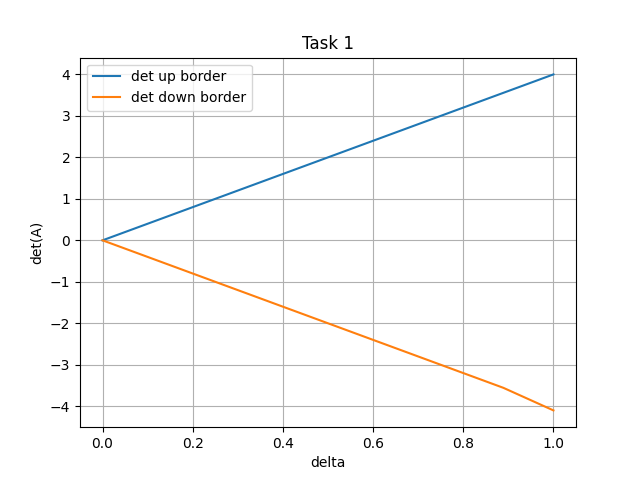
\includegraphics[width=0.5\linewidth]{task1.png}
\end{figure}
Получается, что $det(X_1)$ содержит 0 при $\delta \geqslant 0.05128$
\subsubsection{критерий Баумана}
Множество $\mathrm{vert}(\textbf{A})$ состоит из 4 элементов:
\begin{equation}
\mathrm{vert}(X_1)=
   \biggl\{
        \begin{pmatrix}
        1.05 \pm \delta & 1 \\
        0.95 \pm \delta & 1
        \end{pmatrix}
        \biggl\}
\end{equation}
Получим таблицу результатов для некотрых $\delta$
\begin{table}[H]
\begin{center}
\begin{tabular}{|c|c|}
\hline
$\delta$ & особенность матрицы \\
\hline
0.051273    &    неособенная\\
0.051276    &    неособенная\\
0.051279    &    неособенная\\
0.051282    &    неособенная\\
0.051285    &    особенная\\
0.051288    &    особенная\\
0.051291    &    особенная\\
0.051294    &    особенная\\
\hline
\end{tabular}
\end{center}
\end{table} 
Таким образом, матрица особенная при $\delta \geqslant 0.051285$


\subsection{Задача томографии}
\subsubsection{Графический способ}
Определитель матрицы 2х2 :
\begin{center}
    $det(A) = a_{11}a_{22} - a_{21}a_{12}$
\end{center}
Получим гарфик нижней и верхней границы интервала при $\delta \in [0,1]$:
\begin{figure}[H]
        \centering
        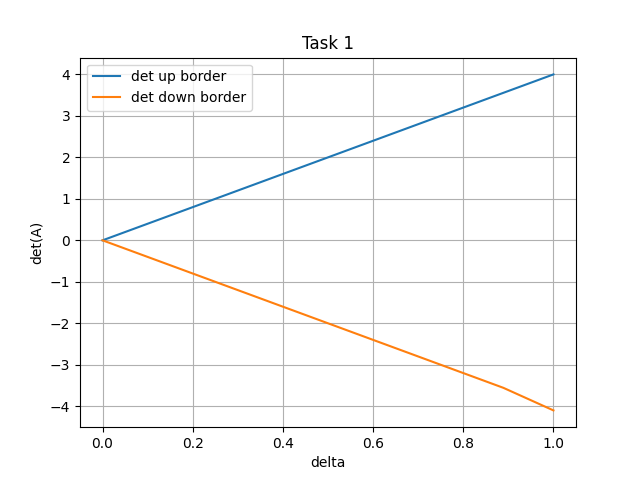
\includegraphics[width=0.5\linewidth]{task1.png}
\end{figure}
Получается, что $det(X_2)$ содержит 0 при $\delta > 0.025$
\subsubsection{критерий Баумана}
Множество $vert(X_2)$ состоит из 16 элементов:
\begin{equation}
\mathrm{vert}(X_2)=
   \biggl\{
        \begin{pmatrix}
        1.05 \pm \delta & 1 \pm \delta \\
        0.95 \pm \delta & 1\pm \delta
        \end{pmatrix}
        \biggl\}
\end{equation}
Получим таблицу результатов для некотрых $\delta$
\begin{table}[H]
\begin{center}
\begin{tabular}{|c|c|}
\hline
$\delta$ & особенность матрицы \\
\hline
0.02473 &   неособенная\\
0.02482 &   неособенная\\
0.02491 &   неособенная\\
0.02500  &  неособенная\\
0.02509 &   особенная\\
0.02518  &  особенная\\
0.02527  &  особенная\\
0.02536  &  особенная\\
\hline
\end{tabular}
\end{center}
\end{table} 
Таким образом, матрица особенная при при $\delta > 0.025$



\section{Вывод}
Данные матрицы $X_1$,$\;X_2$  являются  неособенной при $\delta < 0.051285$ и $\delta \le 0.025$. С помощью критерия Баумана можно получить более точный результат.\\ 
В задаче регресии мы получаем более широкий интервал для $\delta$, чем в задаче томографии.
\end{document}